% Explain the background and theory underlying your project.
% Assume that the average reader has the same knowledge you had \emph{before} undergoing this project.
% This chapter should transfer all knowledge necessary to understand the following chapters.

% As this and the following chapters are likely longer than a few pages, consider structuring them into sections (but avoid fragmentation by overly fine-grained sectioning).
% Use the \verb|\..section{}| command family as illustrated below:


% Follow a top-down approach when structuring the chapter, and guide the reader by giving a short overview at the beginning of each section.
% Again, you can use labels and references (e.g., referring to \cref{sec:background_overview}).

\chapter{Background}
\label{ch:background}

This chapter covers what is needed to follow the rest of the report. \Cref{sec:background_pedals} describes the distortion effects modeled in this work and why they are difficult to model. \Cref{subsec:background_pwh} introduces the \gls{pwh} model, and \cref{sec:background_identification} the multisine measurements and error measures used to identify and evaluate it. \Cref{sec:background_realtime} covers the constraints of running such a model in real time and introduces the graetli.


\section{Guitar distortion pedals}
\label{sec:background_pedals}

A distortion pedal amplifies the guitar signal and then limits it, usually with diodes or transistors. The limiting creates harmonics, which give the effect its sound. Filters before and after the clipping stage shape which frequencies are distorted and how bright the result sounds.

\subsection{Why distortion is difficult to model}
\label{subsec:background_hard_to_model}

Three properties make distortion difficult to model:
\begin{itemize}
  \item \textbf{Memory:} Coupling capacitors, the frequency-dependent gain of the op-amp stage and the tone filter mean that the output depends on past input, not only on the current sample. Since filters sit both before and after the clipping, the circuit cannot be reduced to a static curve.
  \item \textbf{Level dependence:} A quiet note passes almost linearly, while a hard pick is clipped. The tone therefore changes with playing dynamics, and a model fitted at one level does not hold at another.
  \item \textbf{Aliasing:} Clipping creates harmonics far above the audio band. In the analog circuit they are simply attenuated. In a model running at \SI{48}{\kilo\hertz}, harmonics above \SI{24}{\kilo\hertz} fold back into the audible range~\cite{parker2016adaa}.
\end{itemize}

\subsection{JHS -- Packrat}
\label{subsec:background_packrat}

The Packrat~\cite{jhs_packrat} (\cref{fig:packrat}) is based on the ProCo RAT~\cite{proco_rat}. The input goes to an op-amp gain stage whose gain is set by the distortion knob. Two diodes to ground then clip the signal hard. A passive RC low-pass (the filter knob) and a volume control follow. A rotary switch selects between nine variants of the RAT circuit, which differ mainly in the clipping diodes and the gain stage.


\subsection{Greuter Audio -- Natural Selection}
\label{subsec:background_natural_selection}

Natural Selection (\cref{fig:natural_selection}) is an overdrive pedal, hand-built in Switzerland~\cite{greuter_natural_selection}. Compared to the Packrat, it is designed for a more transparent, lower-gain sound that preserves the character of the guitar and amplifier. A JFET input stage drives an op-amp gain stage with diode clipping, followed by an active three-band equalizer. Two clipping options are available: an asymmetric arrangement of silicon diodes, and a symmetric combination of germanium and silicon diodes, which compresses more and sounds closer to a fuzz. The supply voltage is doubled internally to increase the headroom.

\begin{figure}[htbp]
  \centering
  \begin{subfigure}[b]{0.4\textwidth}
    \centering
    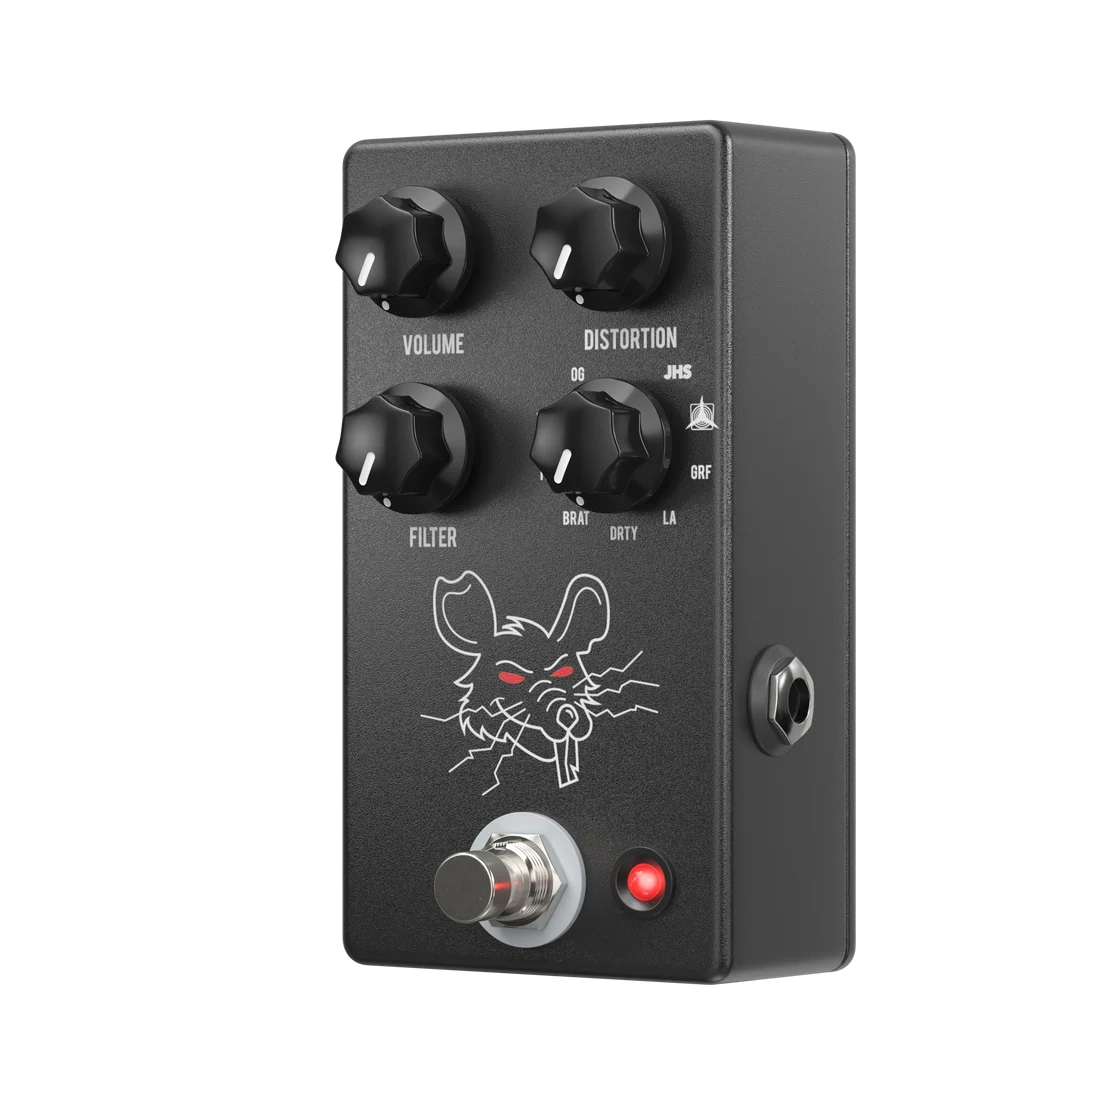
\includegraphics[width=\textwidth]{img/Packrat.png}
    \caption{JHS -- Packrat~\cite{jhs_packrat}}
    \label{fig:packrat}
  \end{subfigure}
  \hfill
  \begin{subfigure}[b]{0.4\textwidth}
    \centering
    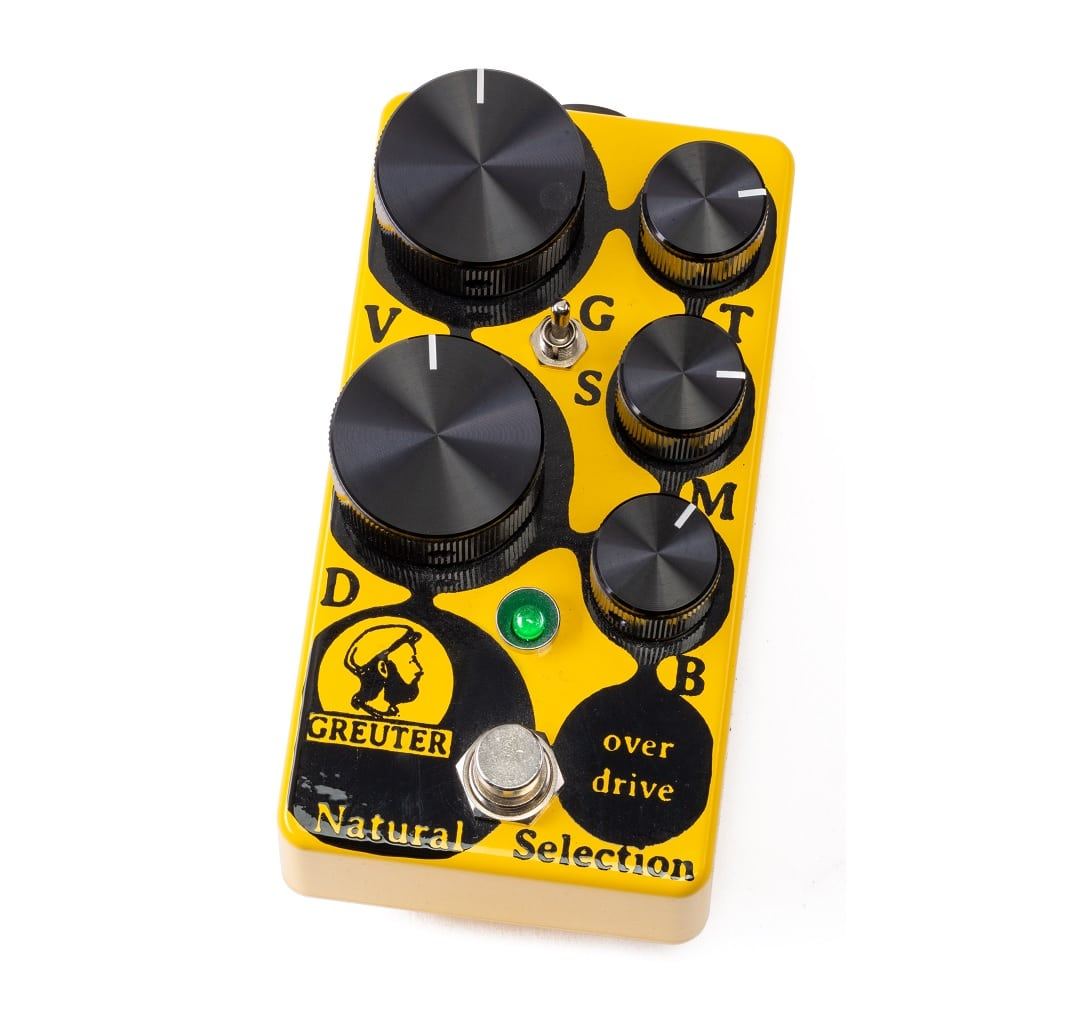
\includegraphics[width=\textwidth]{img/NaturalSelection.jpg}
    \caption{Greuter -- Natural Selection~\cite{greuter_natural_selection}}
    \label{fig:natural_selection}
  \end{subfigure}
  \caption{Analog pedals modeled in this work.}
  \label{fig:pedals}
\end{figure}

\subsection{Other effects}
\label{subsec:background_other_effects}

To test the method before measuring real hardware, we used PeakEater~\cite{peakeater}, an open-source clipping plugin, and ran it offline. Because it is a plugin, it gives noise-free data and can be reproduced exactly.



\section{Parallel Wiener--Hammerstein (PWH)}
\label{subsec:background_pwh}

A Wiener--Hammerstein system is a linear filter, followed by a static nonlinearity, followed by a second linear filter. It matches the structure of a distortion pedal quite directly: a filter before the clipping, the clipping itself, and the tone filter after it. A single branch, however, has one fixed nonlinearity between two fixed filters, and cannot capture how the frequency response of the device changes with level. The \gls{pwh} model (\cref{fig:pwh_structure}) therefore sums $K$ such branches~\cite{schoukens2015pwh}:
\begin{equation}
  y[n] = \sum\sb{i=1}^{K} \big(h\sb{\mathrm{b},i} * f\sb{i}(h\sb{\mathrm{f},i} * x)\big)[n],
  \label{eq:pwh}
\end{equation}
where $h\sb{\mathrm{f},i}$ and $h\sb{\mathrm{b},i}$ are the front and back filters of branch $i$ and $f\sb{i}$ is its static nonlinearity. With several branches, each with its own filters and nonlinearity, the model can represent a response that changes with level.

In the framework used in this work~\cite{pwh_pa_code}, all filters share one set of poles. The poles are taken from \glspl{bla} measured at several input levels (\cref{subsec:background_bla}). Each branch receives a subset of these poles and zeros for its front filter and the rest for its back filter. Finding a good split is a combinatorial search over the possible partitions. The nonlinearities $f\sb{i}$ are then fitted to the measured data. In this work, we additionally refine the whole model with gradient descent and represent each $f\sb{i}$ as a uniform cubic spline instead of a polynomial (\cref{subsec:background_splines}).

\begin{figure}[htbp]
  \centering
  \begin{tikzpicture}[
    block/.style={draw, rectangle, minimum width=1.5cm, minimum height=0.8cm, align=center},
    sum/.style={draw, circle, inner sep=1pt, minimum size=0.6cm},
    >={Stealth}, node distance=0.7cm and 0.8cm
  ]
    % Branches
    \node[block] (f1) {$h\sb{\mathrm{f},1}$};
    \node[block, right=of f1] (n1) {$f\sb{1}(\cdot)$};
    \node[block, right=of n1] (b1) {$h\sb{\mathrm{b},1}$};
    \node[block, below=of f1] (f2) {$h\sb{\mathrm{f},2}$};
    \node[block, right=of f2] (n2) {$f\sb{2}(\cdot)$};
    \node[block, right=of n2] (b2) {$h\sb{\mathrm{b},2}$};
    \node[below=0.35cm of n2] {$\vdots$};
    \node[block, below=1.1cm of f2] (fK) {$h\sb{\mathrm{f},K}$};
    \node[block, right=of fK] (nK) {$f\sb{K}(\cdot)$};
    \node[block, right=of nK] (bK) {$h\sb{\mathrm{b},K}$};

    % Input split
    \coordinate (split) at ($(f1.west)!0.5!(fK.west) + (-1.0,0)$);
    \node[left=0.8cm of split] (x) {$x[n]$};
    \fill (split) circle (1.5pt);
    \draw (x) -- (split);
    \foreach \i in {1,2,K} {
      \draw[->] (split) |- (f\i.west);
      \draw[->] (f\i) -- (n\i);
      \draw[->] (n\i) -- (b\i);
    }

    % Sum and output
    \node[sum] (s) at ($(b1.east)!0.5!(bK.east) + (1.2,0)$) {$+$};
    \foreach \i in {1,2,K} \draw[->] (b\i.east) -- (s);
    \node[right=0.8cm of s] (y) {$y[n]$};
    \draw[->] (s) -- (y);
  \end{tikzpicture}
  \caption{Structure of the \gls{pwh} model with $K$ branches, each consisting of a front filter $h\sb{\mathrm{f},i}$, a static nonlinearity $f\sb{i}$ and a back filter $h\sb{\mathrm{b},i}$.}
  \label{fig:pwh_structure}
\end{figure}
\section{System identification with multisines}
\label{sec:background_identification}

The \gls{pwh} model is identified from measurements with a designed test signal, not from recorded guitar playing. This section introduces the test signal, the \gls{bla} estimated from it, and the error measures used to compare model and device.


\subsection{Random-phase multisines, periods and realizations}
\label{subsec:background_multisines}

A random-phase multisine is a sum of sines whose frequencies lie exactly on a chosen set $\mathcal{K}$ of \acrfull{dft} bins, i.e., on multiples of $f\sb{s}/N$~\cite{pintelon2012sysid}:
\begin{equation}
  x[n] = \sum\sb{k \in \mathcal{K}} A\sb{k} \cos\!\left(\frac{2\pi k n}{N} + \varphi\sb{k}\right),
  \label{eq:multisine}
\end{equation}
where the phases $\varphi\sb k$ are drawn uniformly from $[0, 2\pi)$. The signal is periodic with period $N$, so its spectrum has no leakage, and the frequency resolution is $f\sb{s}/N$. The amplitudes $A\sb{k}$ set the spectrum. We place the bins logarithmically, so that each octave receives about the same power. Each \emph{realization} uses new random phases and is played for $P$ periods. The first period lets transients die out and is discarded. The variation between periods of one realization is measurement noise. The additional variation between realizations comes from the nonlinearity. Repeating the measurement at several RMS levels shows how the device changes with level.

\subsection{Best linear approximation (BLA) and its level dependence}
\label{subsec:background_bla}

For a given input spectrum and level, the \gls{bla} $G\sb{\mathrm{BLA}}(k)$ is the linear system that best approximates the nonlinear device in the least-squares sense~\cite{pintelon2012sysid}. The output then splits into
\begin{equation}
  Y(k) = G\sb{\mathrm{BLA}}(k)\, X(k) + Y\sb{\mathrm{S}}(k) + N\sb{Y}(k),
  \label{eq:bla}
\end{equation}
where $Y\sb{\mathrm{S}}$ are the stochastic nonlinear distortions, which behave like noise across realizations, and $N\sb{Y}$ is the measurement noise. The \gls{bla} is estimated by averaging $Y(k)/X(k)$ over the realizations. The spread across periods and realizations gives the variance of $N\sb{Y}$ and $Y\sb{\mathrm{S}}$. For a linear device the \gls{bla} does not depend on the input. For a distortion pedal it changes with the input level: as the pedal clips harder, its gain drops and its frequency response changes. The \gls{pwh} identification relies on this change to find its branches (\cref{subsec:background_pwh}).


\section{Error measures}
\label{sec:background_error_measures}

To compare the model with the device, we use three error measures. The \gls{nmse} compares the waveforms sample by sample, while the \gls{mrstft} loss and the weighted spectral distance compare magnitude spectrograms and therefore ignore inaudible phase differences.

\subsection{Normalized mean squared error (NMSE)}
\label{subsec:background_nmse}

The \gls{nmse} compares the model output $\hat{y}$ with the measured output $y$ sample by sample:
\begin{equation}
  \mathrm{NMSE} = 10 \log\sb{10} \frac{\sum\sb{n} |y[n] - \hat{y}[n]|^2}{\sum\sb{n} |y[n]|^2}\ \mathrm{dB}.
  \label{eq:nmse}
\end{equation}
It is strict: a small delay or phase shift, which is inaudible, already raises it. When an overall level difference is not of interest, we also report a gain-matched \gls{nmse}, where $\hat{y}$ is first scaled by the least-squares gain $g = \sum\sb{n} y\hat{y} / \sum\sb{n} \hat{y}^2$.

\subsection{Multi-resolution STFT loss}
\label{subsec:background_mrstft}

The \gls{mrstft} loss one of the standard spectral losses in neural audio-effect modeling and natural language processing~\cite{yamamoto2020pwg, steinmetz2020auraloss, comunita2025differentiable}. Like the spectral distance, it compares magnitude spectrograms, but at several time--frequency resolutions at once. For one STFT resolution $m$, it combines a spectral convergence term and a log-magnitude term:
\begin{align}
  \mathcal{L}\sb{\mathrm{sc}}^{(m)} &= \frac{\big\| |Y\sb{m}| - |\hat{Y}\sb{m}| \big\|\sb{\mathrm{F}}}{\big\| |Y\sb{m}| \big\|\sb{\mathrm{F}}}, \label{eq:sc_loss} \\
  \mathcal{L}\sb{\mathrm{mag}}^{(m)} &= \frac{1}{T\sb{m} F\sb{m}} \big\| \log |Y\sb{m}| - \log |\hat{Y}\sb{m}| \big\|\sb{1}, \label{eq:mag_loss}
\end{align}
where $Y\sb{m}$ and $\hat{Y}\sb{m}$ are the STFTs of the measured and the model output with $T\sb{m}$ frames and $F\sb{m}$ frequency bins, and $\|\cdot\|\sb{\mathrm{F}}$ is the Frobenius norm. The spectral convergence term emphasizes the strong spectral components, while the log-magnitude term also weights quiet components such as the high harmonics. The total loss averages over $M$ resolutions:
\begin{equation}
  \mathcal{L}\sb{\mathrm{MR}} = \frac{1}{M} \sum\sb{m=1}^{M} \Big( \mathcal{L}\sb{\mathrm{sc}}^{(m)} + \mathcal{L}\sb{\mathrm{mag}}^{(m)} \Big).
  \label{eq:mrstft}
\end{equation}
We compute the loss with a NumPy reimplementation of the \texttt{MultiResolutionSTFTLoss} of auraloss~\cite{steinmetz2020auraloss}, using its default settings: FFT sizes of 512, 1024 and 2048 samples ($M = 3$) with Hann windows of 240, 600 and 1200 samples. A loss of 0 means identical spectrograms; lower values are better. This allows a comparison with neural models evaluated with the same metric.

\subsection{Weighted spectral distance}
\label{subsec:background_spectral_distance}

The spectral distance compares magnitude spectrograms and ignores the phase. For one STFT window length, it is the mean of
\begin{equation}
  d(f, t) = \left| 20 \log\sb{10} \frac{|\hat{Y}(f,t)| + \epsilon}{|Y(f,t)| + \epsilon} \right| \ \mathrm{dB}
  \label{eq:specdist}
\end{equation}
over time, followed by a weighted average over frequency. The weight $w(f) = A(f)/f$ counts each octave equally and then applies the A-weighting $A(f)$ of the ear~\cite{iec61672}. The floor $\epsilon$ lies \SI{60}{\decibel} below the peak of $|Y|$, so that nearly silent bins do not dominate. The final value averages three window lengths (256, 1024 and 4096 samples). Short windows capture the attack and long ones the tone. A distance of \SI{0}{\decibel} means identical spectrograms.

\section{Real-time audio on embedded hardware}
\label{sec:background_realtime}

A pedal has to produce its output while the guitarist plays, without audible delay and without dropouts. This section explains how embedded audio is processed, how the two building blocks of the \gls{pwh} model are computed, and which platform they run on.

\subsection{Block processing, latency and time budget}
\label{subsec:background_block_processing}

Audio is not processed sample by sample but in blocks of $B$ samples. The audio codec fills one buffer while the processor works on the previous one. This adds a latency of at least one block on the input and one on the output, on top of the delay of the converters. In return, every block must be finished before the next one arrives:
\begin{equation}
  T\sb{\max} = \frac{B}{f\sb{s}}.
  \label{eq:budget}
\end{equation}
At $B = 32$ and $f\sb{s} = \SI{48}{\kilo\hertz}$ this gives \SI{667}{\micro\second} per block, or about \SI{0.7}{\milli\second} of latency per block. A larger block relaxes neither the budget per sample nor the total work, but adds latency. The model and the firmware therefore have to fit within $T\sb{\max}$.

\subsection{Biquad filters on a DSP}
\label{subsec:background_biquads}

The filters of the \gls{pwh} model are implemented as cascades of second-order sections, or biquads:
\begin{equation}
  H(z) = \frac{b\sb{0} + b\sb{1} z^{-1} + b\sb{2} z^{-2}}{1 + a\sb{1} z^{-1} + a\sb{2} z^{-2}}.
  \label{eq:biquad}
\end{equation}
In the time domain, each section computes the difference equation
\begin{equation}
  y[n] = b\sb{0}\, x[n] + b\sb{1}\, x[n-1] + b\sb{2}\, x[n-2] - a\sb{1}\, y[n-1] - a\sb{2}\, y[n-2],
  \label{eq:biquad_diff}
\end{equation}
and the output of one section is the input of the next. A high-order filter evaluated as a single section is sensitive to rounding in single precision. In practice, higher-order filters are therefore usually implemented as cascades of biquads~\cite{zoelzer2011dafx}. Each biquad needs five multiplications per sample.

\subsection{Splines on a DSP}
\label{subsec:background_splines}

For the nonlinearity, a polynomial is the obvious choice. A polynomial of degree $P$ is evaluated efficiently with Horner's rule, which nests the terms so that no powers have to be computed. This costs one multiplication and one addition per degree. However, a hard clipping curve has a sharp knee and flat regions, and a single polynomial needs a high degree to follow it. Fitting it is then numerically sensitive, and outside the fitted range the polynomial quickly diverges.\\

A spline avoids this by splitting the input range into intervals and using a separate low-degree polynomial on each interval~\cite{deboor2001splines}. The interval boundaries are called knots. In a spline of degree $D$, each piece is a polynomial of degree $D$, and neighboring pieces are joined so that the curve and its first $D-1$ derivatives are continuous at the knots. Cubic splines ($D = 3$) are the most common choice, as they are the lowest degree with a continuous second derivative. The result is smooth, but each piece only has to describe a small part of the curve, so a sharp knee can be followed without a high degree.

In a \emph{uniform} spline, the knots are equally spaced with width $\Delta$ over the range $[x\sb{\min}, x\sb{\max}]$. To evaluate it, the input is first clamped to this range. The interval index $i$ and the position $t \in [0, 1)$ within the interval follow directly from the input:
\begin{equation}
  u = \frac{x - x\sb{\min}}{\Delta}, \qquad i = \lfloor u \rfloor, \qquad t = u - i.
  \label{eq:spline_index}
\end{equation}
The polynomial of interval $i$ is then evaluated with Horner's rule:
\begin{equation}
  f(x) = c\sb{0,i} + t\Big(c\sb{1,i} + t\big(c\sb{2,i} + \dots + t\, c\sb{D,i}\big)\dots\Big).
  \label{eq:spline_eval}
\end{equation}
Apart from the index computation, this costs $D$ multiplications, three for a cubic spline, regardless of how many intervals the spline has. More intervals only increase the size of the coefficient table in memory. In this work uniform cubic splines are used.


\subsection{graetli}
\label{subsec:graetli}

The graetli is a guitar pedal platform built at ETH by Silvan Krebs and Jonas Roth~\cite{graetli_krebs}. At its core is an Electrosmith Daisy Seed, with an STM32H750 microcontroller. Its Arm Cortex-M7 core has a single-precision floating-point unit and runs at \SI{400}{\mega\hertz} in our configuration. Around the Daisy Seed, the graetli adds input and output jacks, a relay for analog bypass, potentiometers, footswitches, buttons, an encoder and a small display. The firmware is written in C++ on top of libDaisy and builds on a test firmware by Jonas Roth.~\cite{graetli_krebs}\\

The audio runs at \SI{48}{\kilo\hertz} with blocks of 32 samples, so the budget of \cref{eq:budget} is \SI{667}{\micro\second}. A second limit is memory: the program has to fit into the \SI{128}{\kilo\byte} of internal flash. Finally, the full scale of the graetli's converters differs from that of the audio interface used for the measurements. A model identified on recorded data therefore needs an input and an output gain on the graetli to see the same signal levels (\cref{subsec:impl_calibration}).

\begin{figure}[htbp]
  \centering
  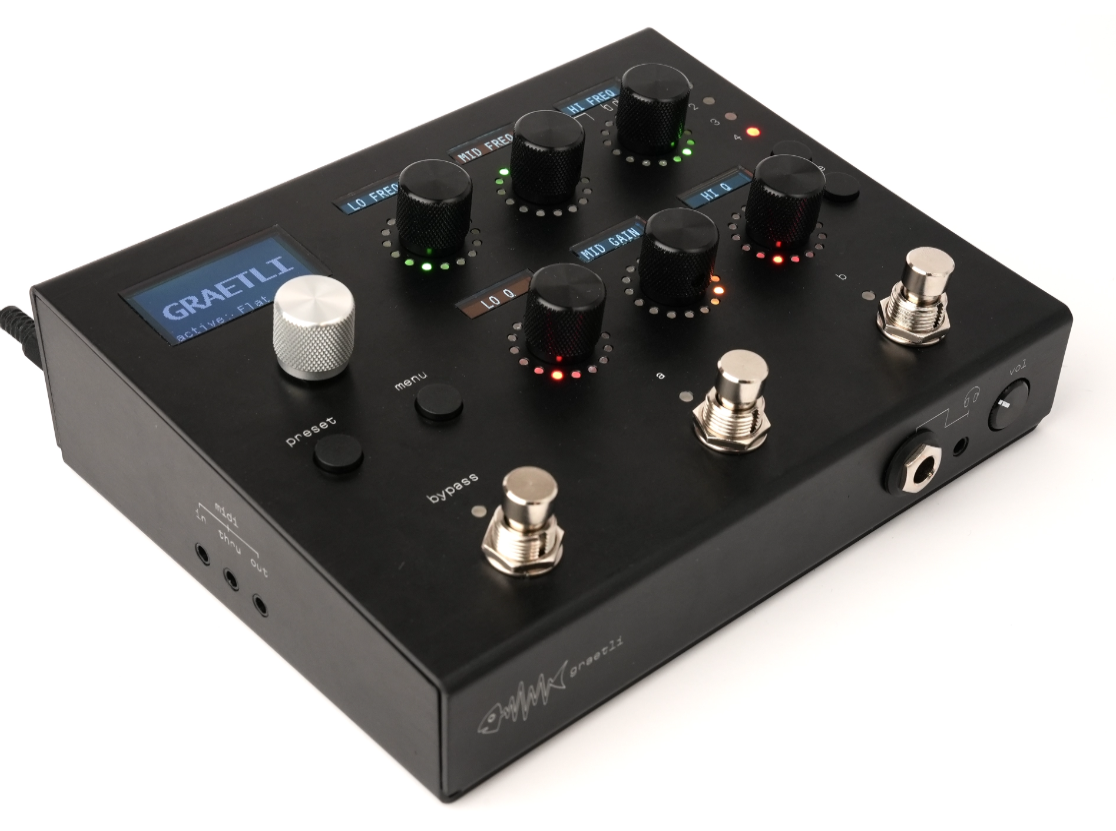
\includegraphics[width=0.6\textwidth]{img/graetli.png}
  \caption{The graetli by Silvan Krebs.~\cite{graetli_krebs}}
  \label{fig:packrat}
\end{figure}